

\section{Einleitung}

Aufgrund gewünschten Portabilität oder Skalierbarkeit kann es möglich sein das der Wunsch besteht Legacy Software zu containerisieren. In diesem Kapitel wird kurz auf die begriffe Legacy sowie Containerisierung eingegangen.

\subsubsection{Legacy - Software}
Der Begriff Legacy - Software wird in der Informatik oft im engeren Sinne mit einer historisch gewachsenen Anwendung und oder als Altlast, Hinterlassenschaft verwendet. (Michael C Feathers) schrieb dazu: Das in der Branche Legacy Code oftmals als schwer zu änderbaren oder nicht verständlicher Code bezeichnet wird. ~\cite{feathers2020effektives}
Dies kann dann z.B auftreten wenn man aus kostengründe software einkauft welche nicht quelloffen ist welche dann mit den jahren nicht an die eigenen anforderungen angepasst wird oder
aus oben genannten kostengründen nicht angepasst werden soll.

\subsubsection{Containerisierung}
die containerisierung wird in der informatik verwendet um die virtualisierung einer laufzeitumgebung mittels software zu gewährleisten. hierfür wird oftmals Docker verwendet, einem containerisierungs tool welches container erstellen kann die alle notwendige abhängigkeiten besitzen um
software unabhängig zu betreiben. die funktionsweise von docker lässt sich folgendermaßen erklären, anstelle wie bei virtuellen maschinen die einen hypervisor benutzen um die befehle des instanzierten betriebssystems übersetzen
auf die des host systems, laufen container direkt auf dem host system.

\begin{figure}[h]
	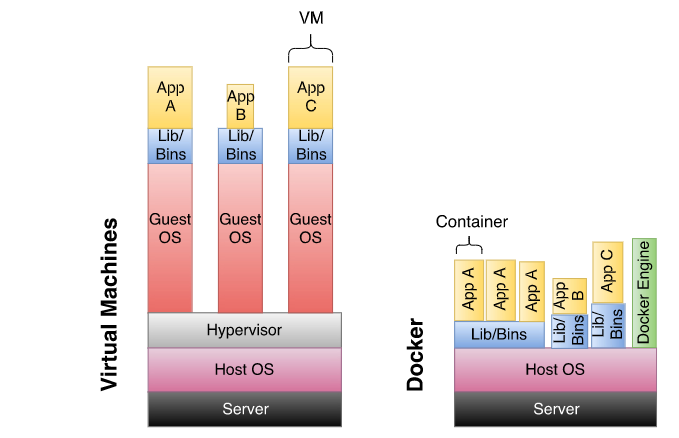
\includegraphics[width=\columnwidth]{gfx/vm vs container.png} %.5\textwidth
	\caption{Unterschied zwischen Virtualisierung und Container, Quelle: Albin Sundqvist \cite{sundqvist2020guidelines}}
\end{figure}

Ein weitere Vorteil von Container ist das man sie so konfigurieren kann das sie ausschließlich für die Software benötigten
Abhängigkeiten besitzt und nicht den ganzen overhead einer virtualisierung. Die erstellung solcher container erfolgt mittels images, dieses beinhalte read-only informationen die für die erstellung eines containers notwendig sind. images werden in layer definiert. Diese
layer kann man in einer dockerfile definieren, jeder ausgeführte befehl wird als zusätzlicher layer dem image hinzugefügt und es wird ein hashwert gezogen für den späteren gebrauch.

\begin{figure}[h]
	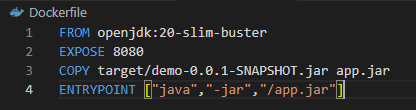
\includegraphics[width=\columnwidth]{gfx/Dockerfile.png} %.5\textwidth
	\caption{Beispiel einer Dockerfile}
\end{figure}

Wird nun also so ein Image erstellt schaut erstmal docker in seinem build cache ob die layer die benötigt werden bereits als hash vorhanden sind und können so wieder verwendet werden.
Weitere informationen lassen sich dies bezüglich aus der Overview of Docker Build \cite{dockerbuild} nachschlagen.

\section{Szenario}

oftmals kann es dazu kommen das man Legacy - Software im betrieb hat welche mehrere Jahre alt ist und teils nicht mehr gewartet wird oder nicht mit den wachsenden anforderungen wächst.
ist diese dann auch noch eine systemkritische komponente kann sie schnell zu einem bottleneck in einem workflow werden. das ersetzen solcher software lässt sich je nach umfang nur mit einem hohen geldaufwand bewerkstelligen.
Da die software weder quelloffen ist noch einfach ausgetauscht werden kann liegt hier der versuch nahe sie zu containerisieren um sie dann anschließend zu skalieren. dies wäre natürlich auch
mittels virtuellen maschinen möglich hierbei ist aber zu beachten das dies einen erhöhten konfigurationsaufwand hätte.

\section{Auftretende Probleme}

aufgrund der komplexiät solcher szenarien ist es mir jetzt nicht möglich auf alle problematiken einzugehen, dennoch möchte ich hier die häufigsten aufgreifen.
während der containerisierung kann man auf diverse probleme stoßen die mitunter den ganzen vorgang erschweren oder sogar unmöglich werden lassen. um dies zu verhindern sollte
man folgende punkte stets kritisch prüfen und schauen ob diese gegen eine containerisierung sprechen.

\begin{description}
	\item[\textbf{Source Code:}]\hfill \\ Bei Legacy Software kann der Source Code in den unterschiedlichsten varianten vorliegen, manchmal auch garnicht. Hier eine auflistung der möglichkeiten. \\
	\begin{itemize}
		\item[(a)] Er ist vorliegend, man hat sogar die möglichkeiten änderungen vorzunehmen. \\
		\item[(b)] teilweise oder ganz vorliegend aber keine mögichkeit änderungen vorzunehmen. \\
		\item[(c)] Source Code liegt nicht vor und somit weder änderbar noch einsehbar. \\
	\end{itemize}
	\item[\textbf{Arbeitsweise der Software:}]\hfill \\ Auch hier gibt es einige punkte die gegen eine Containerisierung sprechen, gerade desktop applications die auf einem frontend aufbauen das zu bedienen gilt fallen hier heraus. der mehraufwand ein solches system in betrieb zu nehmen wäre höher als das aufsetzen einer ganzen VM. daher eignen sich eher Applications die entweder über command line argumente annehmen oder beim start ihre arbeit von selbst verrichten ohne weiteres zutun. \\
	\item[\textbf{Installation:}]\hfill \\ Hier gilt ähnlich bei der Arbeitsweise der Software, eine Software lässt sich sofern sie eine Installation benötigt, nur mit einem erhöhtem Mehraufwand installieren wenn es dafür nur eine grafische oberfläche gibt die man bedienen muss. Hierfür müssten dann alle Installationsschritte händisch (oder mittels script) nachgestellt werden. Gerade bei einem Betriebssystem wie Windows kann dies zu einer äußerst mühsehligen arbeitn werden.\\
	\item[\textbf{Spezielle Abhängigkeiten:}]\hfill \\ Je nach Software kann es sein das spezielle abhängigkeiten vorhanden sind wie z.B \\

	\textbf{lizensen:} \\ Dies ist oft der fall wenn die Software eingekauft wurde. diese können oder müssen entsprechend in den Container integriert werden. \\ \\
	\textbf{Hardware Abhängigkeiten:} \\ Es kann auch schonmal vorkommen das gerade bei gekaufter Software lizensen anhand von diversen Hardware Konfigurationen, Mac Adressen, oder sonstigem erstellt werden und dann nur für diesen Computer freigegeben sind. Dies sind besonders schwierige fälle für die es aber auch Lösungsansätze gibt. \\ \\

	\item[\textbf{Speichern von Daten:}]\hfill \\ Oftmals verarbeiten Programme ja nicht nur Daten sondern speichern diese dann auch, das muss entsprechend im vorfeld klar sein wie und wo die daten gespeichert werden. gerade programme die lokal ihre daten speichern und abrufen sind mit einer standartisierten containerisierung problematisch da container in sich ja zustandslos sind und bei jedem neustart immer wieder den urzustand wieder erhalten. \\
	\item[\textbf{Uvm...}]\hfill \\ wie schon oben beschrieben, gibt es einige mehrere probleme die auftreten können und aufgrund der komplexität dessen werde ich nur ein paar Lösungsansätze für die oben beschrieben probleme angehen. \\
\end{description}

\section{Lösungsansätze}

\begin{description}
	\item[\textbf{Source Code}]\hfill \\


	\textbf{Quelloffen:}\\ Dies ist sehr unproblematisch, man kann das Verhalten der Software nachvollziehen und ggf sogar ändern. \\  \\
	\textbf{Nicht Quelloffen aber Dokumentiert:}\\ Hier lassen sich keine zwar keine änderungen vornehmen aber man kann entsprechend der Dokumentationsqualität das verhalten nachvollziehen und sich darauf entsprechend einstellen bzw. den Container entsprechend anpassen. \\ \\
	\textbf{Nicht Quelloffen und nicht Dokumentiert:}\\ Da weder Sourcecode nocht Dokumentation vorhanden ist, gibt es hier leider nur zwei möglichkeiten. Den hersteller zu rate ziehen oder durch trial and error oder gar durch reverse engineering \cite{eilam2011reversing} (achtung kann strafrechtliche folgen mit sich ziehen) das verhalten des programmes zu ergründen. \\ \\
	\item[\textbf{Arbeitsweise der Software}]\hfill \\ Wie schon bereits im unterpunkt \textbf{Auftretende Probleme} beschrieben macht es natürlich wenig sind software zu containerisieren die trotzdem noch händisch bedient werden muss. dies ist auch ein klarer auscheidepunkt für die containerisierung da ja immernoch personal benötigt wird um es zu bedienen und der mehraufwand dies zu bewerkstelligen höher als der nutzen wäre. dennoch möchte ich hier kurz eine möglichkeiten aufzeigen. Software die ein Webfrontend besitzen kann man natürlich nicht nur prima containerisierung sondern auch mittels Puppeteer \cite{puppeteer} vollautomatisch bedienen lassen. \\ \\
	\item[\textbf{Installation}]\hfill \\ Auch hier ist es äußerst problematisch wenn software über eine installations routine verfügt durch die man sich durch klicken muss. gerade im windows umfeld erlebt man dies ja sehr häufig. abhilfe dafür gibt es, gerade auch windows software besitzt oft eine möglichkeit der installation via command line interface. Für die Windows Microsoft Standard Installer in kurz msi files gibt es folgende Website die man zu rate ziehen kann:\textbf{Microsoft Standard Installer Command-Line Optionen} \cite{microsoft} oder folgende seite die nicht nur Microsoft bezogen ist: \textbf{Silent Install HQ} \cite{Silent}  die einem mit genügend Tutorials versorgt um die entsprechende Software dann doch zu installieren.\\ \\
	\item[\textbf{Spezielle Abhängigkeiten}]\hfill \\ Wie schon oben beschrieben, müssen Lizensen in die entsprechenden Container integriert werden. Handelt es sich hier um simple Lizensdateien kann man diese COPY oder ADD \cite{dockerbuild} in der Dockerfile hinzufügen. Schwierigier wird es hingegen wenn wirklich Hardware abhängigkeiten bestehen. Zwar lassen sich Docker Container hier vielfältig anpassen z.B die Mac oder IP Adresse, siehe \cite{dockerrunnetwork}. Aber auch hier gibt es gewisse beschränkungen da so ein Container nicht endlos anpassbar ist. Sollten hier probleme auftreten aufgrund eines gesonderten Authentisierungsverfahren sollte man den Betreiber der Software möglichst zu rate ziehen. \\ \\
	\item[\textbf{Speichern von Daten:}]\hfill \\ Da Container an sich Zustandslos sind wäre es äußerst unvorteilhaft wenn alle daten die zu speichern sind nach dem neustart verloren wären. hierfür hat docker aber eine lösung, in der Dokumentation unter \textbf{Manage data in Docker} \cite{dockerrstorage} wird beschrieben wie man nicht flüchtigen speicher an container anbindet. Dieses problem tritt natürlich nicht bei Container auf die nur Daten verarbeiten und dann weiter geben, hier ist nur darauf zu achten das im falle eines absturzes die Arbeit am richtigen punkt wieder aufgenommen wird.\\ \\
\end{description}

\section{Zusammenfassung und Ausblick}

In dieser Arbeit werden die Herausforderungen bei der Containerisierung von Legacy-Software untersucht. Legacy-Software wird in der Informatik oft als historisch gewachsene Anwendung oder als Altlast, Hinterlassenschaft, bezeichnet. Dies kann vorkommen, wenn Software aus Kostengründen eingekauft wird, die nicht quelloffen ist und im Laufe der Zeit nicht an die eigenen Anforderungen angepasst wird. Eine Möglichkeit, Legacy-Software zu modernisieren und für eine bessere Portabilität und Skalierbarkeit fit zu machen, ist die Containerisierung.

Containerisierung ist eine Technologie, die in der Informatik verwendet wird, um die Virtualisierung einer Laufzeitumgebung mittels Software zu gewährleisten. Ein gängiges Tool zur Containerisierung ist Docker, das Container erstellen kann, die alle notwendigen Abhängigkeiten besitzen, um Software unabhängig auszuführen. Der Vorteil von Containern ist, dass sie so konfiguriert werden können, dass sie nur die für die Software erforderlichen Abhängigkeiten besitzen und nicht den gesamten Overhead einer Virtualisierung.

In dieser Arbeit wird aufgezeigt, welche Anforderungen an die zu containerisierende Software bestehen und welche Probleme und Einschränkungen innerhalb eines Windows-Umfelds auftreten können. Es wird gezeigt, dass die Containerisierung von Legacy-Software eine Herausforderung darstellt, insbesondere in Bezug auf die Anpassung an die Anforderungen des Host-Systems und die Behandlung von Abhängigkeiten. Es wird auch diskutiert, wie die Erstellung von Images für Container durchgeführt wird und wie die Verwendung von Dockerfiles dazu beitragen kann, den Prozess der Containerisierung zu vereinfachen.

Insgesamt zeigt diese Arbeit, dass die Containerisierung von Legacy-Software eine Herausforderung darstellt, aber durch den Einsatz von Tools wie Docker und durch die Berücksichtigung bestimmter Anforderungen und Einschränkungen erfolgreich durchgeführt werden kann. Es wird empfohlen, die Containerisierung von Legacy-Software sorgfältig zu planen und durchzuführen, um die Vorteile von besserer Portabilität und Skalierbarkeit zu nutzen, ohne dabei die Funktionsfähigkeit der Software

zu beeinträchtigen. Weiterhin wird darauf hingewiesen, dass es wichtig ist, die Anforderungen an die containerisierte Legacy-Software genau zu definieren und sicherzustellen, dass die Containerumgebung alle notwendigen Ressourcen und Abhängigkeiten bereitstellt, damit die Software ordnungsgemäß funktioniert. Es wird auch darauf hingewiesen, dass es wichtig ist, die Sicherheitsaspekte der containerisierten Legacy-Software zu berücksichtigen und sicherzustellen, dass sie auf dem neuesten Stand der Technik sind.

\section{Zur Person}

Name: Andreas Scheuer

Matrikelnummer: 3849139

Studiengang: Praktische Informatik

Mail: pib.andreas.scheuer@htwsaar.de